%! Author = chtompki
%! Date = 1/14/26
\documentclass[12pt]{amsart}
% Default margins are too wide all the way around. I reset them here
\setlength{\hoffset}{-.75in}
\setlength{\textwidth}{6.5in}
\setlength{\voffset}{-.5in}
\setlength{\textheight}{9.0in}
\usepackage{amsmath}
\usepackage{leftindex}
\usepackage{amssymb}
\usepackage{mathrsfs}
\usepackage{tikz}
\usepackage{amsthm}
\usepackage{enumitem}
\usepackage{setspace}
\usetikzlibrary{shadows,arrows,shapes,positioning,calc}

\theoremstyle{definition}
\newtheorem{definition}{Definition}

\newenvironment{solution}
{\begin{proof}[Solution]}
{\end{proof}}

\tikzset{
    ell/.style={draw,ellipse,minimum height=6em,minimum width=10em,align=center},
    inner_ell/.style={draw,ellipse,minimum height=4em,minimum width=6em,align=center},
    ellthin/.style={draw,ellipse,minimum height=2em,minimum width=10em,align=center},
    line/.style={-,line width=0.5pt},
    dot/.style = {draw,fill,circle,inner sep=0pt,outer sep=0pt,minimum size=2pt},
    spot/.style = {draw,fill,circle,inner sep=0pt,outer sep=0pt,minimum size=0pt},
}

\title{Combinatorics\\Notes January 29, 2026}
%\author{Rob Tompkins}
\date{\today}

\begin{document}
    \maketitle
    \date{\today}
    \begin{onehalfspace}
        \section{Sterling Numbers. Con't}
        Let $f:M\rightarrow B$ be a function where $M$ is a set of marbles and $B$ is a set of boxes.
        Also let $m = |M|$ and $b = |B|$
        We concern ourselves with the following counts.
        \begin{enumerate}
            \item We want the count of the number of relations from $M$ to $B$:
            \begin{displaymath}
                \text{count} = 2^{|M\times B|} = 2^{|M||B|} = 2^{mb}
            \end{displaymath}
            \item We want the count of the number of general functions from $M$ to $B$ which follows as:
            \begin{displaymath}
                \text{count} = b^m
            \end{displaymath}
            \item With $m\leq b$ we want to count the number of one-to-one functions from $M$ to $B$ which follows
            as:
            \begin{displaymath}
                \text{count} = \leftindex_b P_m
            \end{displaymath}
            \item With $m \leq b$ we want to count the number of onto functions from $M$ to $B$, which follows as:
            \begin{eqnarray*}
                \text{count} & = & b^m - \binom{b}{1}(b-1)^m + \binom{b}{2}(b-2)^m - \binom{b}{3}(b-3)^m + \cdots + (-1)^b\binom{b}{b}(b - b)^m \\
                & = & b! \cdot \frac{1}{b!} \sum_{k=0}^b (-1)^k\binom{b}{k}(b-k)^m = b!\mathcal{S}(m,b)
            \end{eqnarray*}
            \item With $m = b $ we want to count the number of bijections from $M$ to $B$. This follows as
            \begin{displaymath}
                \text{count} = m! = b!
            \end{displaymath}
        \end{enumerate}
        Now we consider the diagram
        \begin{figure}
            \centering
            \begin{tikzpicture}
                \node[spot](a) {};
                \node[spot,right=4cm of a] (b){};
                \node[dot,below=2cm of b] (c){};
                \node[dot,left= 4cm of c] (d){};
                \node[ell,rotate=90] at ($(b)!0.5!(c)$) {};
                \node[ell,rotate=90] at ($(d)!0.5!(a)$) {};
                \draw[->] (d) -- (c);
            \end{tikzpicture}
            \caption{Set mapping}
        \end{figure}
        \begin{figure}
            \centering
            \begin{tikzpicture}
                \node[spot,label=90:$\text{Domain}$] (a) at (-2,2) {};
                \node[spot,label=90:$\text{CoDomain}$] (b) at (2,2) {};
                \node[spot,label=270:$M$] (c) at (2,-2) {};
                \node[spot,label=270:$B$] (d) at (-2,-2) {};
                \node[dot,label=270:$f(m_1)$,label=90:$\text{Image}$] (e) at (2,0) {};
                \node[dot,label=270:$m_1$,label=90:$\text{PreImage}$] (f) at (-2,0) {};
                \draw [->] (-2,0) .. controls (0,0.5) .. (2,0);
                \node[ell,rotate=90] at ($(b)!0.5!(c)$) {};
                \node[ell,rotate=90] at ($(d)!0.5!(a)$) {};
%                \draw[->] (d) -- (c);
            \end{tikzpicture}
            \caption{Set mapping}
        \end{figure}
        \begin{figure}
            \centering
            \begin{tikzpicture}
                \node[dot](a) {};
                \node[dot,right=2cm of a] (b){};
                \node[dot,below=2cm of b] (c){};
                \node[dot,left= 2cm of c] (d){};
                \node[dot,yshift=-1cm] at ($(a)!0.5!(b)$)(e) {};
                \node[dot] at ($(d)!0.5!(a)$)(f){};
                \node[dot] at ($(f)!0.5!(a)$)(g){};
                \node[dot] at ($(f)!0.5!(d)$)(){};
                \node[dot] at ($(d)!0.15!(f)$)(){};
                \node[dot] at ($(d)!0.3!(f)$)(){};
                \node[ellthin] at ($(a)!0.5!(b)$) {};
                \node[ellthin,rotate=90] at ($(b)!0.5!(c)$) {};
                \node[ellthin] at ($(c)!0.5!(d)$) {};
                \node[ellthin,rotate=90] at ($(d)!0.5!(a)$) {};
                \draw[line] (e) -- (a);
                \draw[line] (e) -- (b);
                \draw[line] (e) -- (f);
            \end{tikzpicture}
            \caption{Something here}
        \end{figure}

        \begin{figure}
            \centering
            \begin{tikzpicture}[
                >=Latex,
                every node/.style={font=\small},
                set/.style={draw, thick},
                inner/.style={draw, thick, pattern=north east lines, pattern color=gray!70},
                map/.style={->, thick},
            ]

% Title
                \node[font=\large] at (5,4.2) {Linear Functions};

% --- Domain (left) ---
                \node at (1.8,3.2) {Domain};

% Outer oval M
                \draw[set] (2,1.5) ellipse (1.4 and 2.0);
                \node at (2,-0.8) {$M$};

% Inner shaded oval = kernel
                \draw[inner] (2,1.5) ellipse (0.65 and 1.35);

% Labels on left
                \node[align=left] at (0.0,1.6) {Kernel\\(Nullspace)};
                \node[align=left] at (0.2,2.45) {Pre-image};

% Some sample points in domain
                \fill (1.85,2.1) circle (1.1pt) node[below left] {$m_1$};
                \fill (2.15,1.5) circle (1.1pt) node[below right] {$m_2$};
                \fill (1.95,0.9) circle (1.1pt) node[below left] {$m_3$};

% --- Codomain (right) ---
                \node at (8.2,3.2) {Codomain};

% Outer oval B
                \draw[set] (8,1.5) ellipse (1.4 and 2.0);
                \node at (8,-0.8) {$B$};

% Inner shaded oval = image/range
                \draw[inner] (8,1.5) ellipse (0.75 and 1.15);

% Labels on right
                \node[align=left] at (9.9,2.25) {$f(M)$\\Range};
                \node[align=left] at (9.65,1.55) {Image};

% Some sample points in image
                \fill (7.9,1.95) circle (1.1pt) node[below left] {$f(m_1)$};
                \fill (8.2,1.55) circle (1.1pt);
                \fill (7.85,1.10) circle (1.1pt);

% Label f over arrows
                \node[font=\normalsize] at (5,2.9) {$f$};

% --- Mapping arrows (stylized like your sketch) ---
                \draw[map] (1.85,2.1) .. controls (4.2,2.6) and (6.0,2.3) .. (7.9,1.95);
                \draw[map] (2.15,1.5) .. controls (4.0,1.8) and (6.2,1.9) .. (8.2,1.55);
                \draw[map] (1.95,0.9) .. controls (4.0,1.1) and (6.0,1.2) .. (7.85,1.10);

% A couple extra faint arrows to mimic multiple strands
                \draw[->, thin, gray!60] (2.6,2.6) .. controls (4.6,2.4) and (6.6,2.6) .. (8.6,2.0);
                \draw[->, thin, gray!60] (2.7,0.5) .. controls (4.7,0.9) and (6.7,0.7) .. (8.7,1.1);

% Optional "co-kernel / left nullspace" note (right side)
                \draw[inner] (11.0,2.2) ellipse (0.55 and 0.45);
                \node[align=left] at (12.3,2.2) {Co-kernel\\Left nullspace};

% Note at bottom right
                \node[font=\small] at (10.2,0.2) {Range $\subset$ Codomain};

            \end{tikzpicture}
            \caption{Chat GPT Tikz}
        \end{figure}

        % Gradient Info

        \tikzset {_6h2o4wtd6/.code = {\pgfsetadditionalshadetransform{ \pgftransformshift{\pgfpoint{0 bp } { 0 bp }  }  \pgftransformrotate{0 }  \pgftransformscale{2 }  }}}
        \pgfdeclarehorizontalshading{_weaugwrqa}{150bp}{rgb(0bp)=(0.71,0.74,0.78);
        rgb(37.5bp)=(0.71,0.74,0.78);
        rgb(37.5bp)=(0.51,0.55,0.58);
        rgb(62.410714285714285bp)=(0.31,0.4,0.46);
        rgb(100bp)=(0.31,0.4,0.46)}
        \tikzset{_czeaqdv2k/.code = {\pgfsetadditionalshadetransform{\pgftransformshift{\pgfpoint{0 bp } { 0 bp }  }  \pgftransformrotate{0 }  \pgftransformscale{2 } }}}
        \pgfdeclarehorizontalshading{_2swwhag5a} {150bp} {color(0bp)=(transparent!0);
        color(37.5bp)=(transparent!0);
        color(37.5bp)=(transparent!0);
        color(62.410714285714285bp)=(transparent!73);
        color(100bp)=(transparent!73) }
        \pgfdeclarefading{_xqz0zbkz5}{\tikz \fill[shading=_2swwhag5a,_czeaqdv2k] (0,0) rectangle (50bp,50bp); }
        \tikzset{every picture/.style={line width=0.75pt}} %set default line width to 0.75pt

        \begin{figure}
            \centering
            \begin{tikzpicture}[x=0.75pt,y=0.75pt,yscale=-1,xscale=1]
%uncomment if require: \path (0,300); %set diagram left start at 0, and has height of 300

%Shape: Rectangle [id:dp5233667101372301]
                \path  [shading=_weaugwrqa,_6h2o4wtd6,path fading= _xqz0zbkz5 ,fading transform={xshift=2}] (135,44) -- (631.3,44) -- (631.3,262.2) -- (135,262.2) -- cycle ; % for fading
                \draw   (135,44) -- (631.3,44) -- (631.3,262.2) -- (135,262.2) -- cycle ; % for border

%Shape: Polygon Curved [id:ds556956836823167]
                \draw  [line width=1.5]  (235.3,145.2) .. controls (217.3,135.2) and (198.3,98.2) .. (245.3,76.2) .. controls (292.3,54.2) and (321,89) .. (320.3,87.2) .. controls (320.3,88.2) and (346.3,103.2) .. (342.3,153.2) .. controls (338.3,203.2) and (258.3,250.2) .. (238.3,220.2) .. controls (218.3,190.2) and (253.3,155.2) .. (235.3,145.2) -- cycle ;
%Shape: Polygon Curved [id:ds47340645770050416]
                \draw  [line width=1.5]  (451.3,117.2) .. controls (458.3,106.2) and (504.3,63.2) .. (539.3,97.2) .. controls (574.3,131.2) and (513.3,131.2) .. (543.3,181.2) .. controls (573.3,231.2) and (469.3,223.2) .. (449.3,193.2) .. controls (429.3,163.2) and (444.3,128.2) .. (451.3,117.2) -- cycle ;
%Curve Lines [id:da4785441068178986]
                \draw [line width=1.5]    (283.97,139) .. controls (317.5,113.85) and (358.32,99.41) .. (392.27,97.2) .. controls (424.71,95.09) and (459.04,113.43) .. (478.61,132.5) ;
                \draw [shift={(481.27,135.2)}, rotate = 226.47] [fill={rgb, 255:red, 0; green, 0; blue, 0 }  ][line width=0.08]  [draw opacity=0] (11.61,-5.58) -- (0,0) -- (11.61,5.58) -- cycle    ;
%Curve Lines [id:da03036214425379491]
                \draw [line width=1.5]    (304.71,190.67) .. controls (350.31,221.84) and (447.3,214.45) .. (486.3,185.2) ;
                \draw [shift={(301.3,188.2)}, rotate = 37.69] [fill={rgb, 255:red, 0; green, 0; blue, 0 }  ][line width=0.08]  [draw opacity=0] (11.61,-5.58) -- (0,0) -- (11.61,5.58) -- cycle    ;
%Shape: Circle [id:dp7942098562220739]
                \draw  [fill={rgb, 255:red, 0; green, 0; blue, 0 }  ,fill opacity=1 ] (273.92,144) .. controls (273.92,141.78) and (275.73,139.97) .. (277.95,139.97) .. controls (280.17,139.97) and (281.97,141.78) .. (281.97,144) .. controls (281.97,146.22) and (280.17,148.03) .. (277.95,148.03) .. controls (275.73,148.03) and (273.92,146.22) .. (273.92,144) -- cycle ;
%Shape: Circle [id:dp4174234972144677]
                \draw  [fill={rgb, 255:red, 0; green, 0; blue, 0 }  ,fill opacity=1 ] (486.27,140.2) .. controls (486.27,137.98) and (488.08,136.17) .. (490.3,136.17) .. controls (492.52,136.17) and (494.32,137.98) .. (494.32,140.2) .. controls (494.32,142.42) and (492.52,144.23) .. (490.3,144.23) .. controls (488.08,144.23) and (486.27,142.42) .. (486.27,140.2) -- cycle ;
%Shape: Circle [id:dp9577878414443755]
                \draw  [fill={rgb, 255:red, 0; green, 0; blue, 0 }  ,fill opacity=1 ] (286.95,182) .. controls (286.95,179.78) and (288.75,177.97) .. (290.97,177.97) .. controls (293.2,177.97) and (295,179.78) .. (295,182) .. controls (295,184.22) and (293.2,186.03) .. (290.97,186.03) .. controls (288.75,186.03) and (286.95,184.22) .. (286.95,182) -- cycle ;
%Shape: Circle [id:dp5217310121519758]
                \draw  [fill={rgb, 255:red, 0; green, 0; blue, 0 }  ,fill opacity=1 ] (495.27,181.2) .. controls (495.27,178.98) and (497.08,177.17) .. (499.3,177.17) .. controls (501.52,177.17) and (503.32,178.98) .. (503.32,181.2) .. controls (503.32,183.42) and (501.52,185.23) .. (499.3,185.23) .. controls (497.08,185.23) and (495.27,183.42) .. (495.27,181.2) -- cycle ;

% Text Node
                \draw (197,186) node [anchor=north west][inner sep=0.75pt]  [font=\huge] [align=left] {$\displaystyle T$};
% Text Node
                \draw (567,179) node [anchor=north west][inner sep=0.75pt]  [font=\huge] [align=left] {$\displaystyle W$};
% Text Node
                \draw (380,65) node [anchor=north west][inner sep=0.75pt]  [font=\LARGE] [align=left] {$\displaystyle \ \mathscr{F}\ $};
% Text Node
                \draw (378,214) node [anchor=north west][inner sep=0.75pt]  [font=\LARGE] [align=left] {$\displaystyle \mathscr{F}^{-1}$};


            \end{tikzpicture}
            \caption{Something here}
        \end{figure}
    \end{onehalfspace}
\end{document}
